% Options for packages loaded elsewhere
\PassOptionsToPackage{unicode}{hyperref}
\PassOptionsToPackage{hyphens}{url}
\PassOptionsToPackage{dvipsnames,svgnames,x11names}{xcolor}
%
\documentclass[
  10pt,
  a4paper,
]{scrreprt}
\usepackage{amsmath,amssymb}
\usepackage{iftex}
\ifPDFTeX
  \usepackage[T1]{fontenc}
  \usepackage[utf8]{inputenc}
  \usepackage{textcomp} % provide euro and other symbols
\else % if luatex or xetex
  \usepackage{unicode-math} % this also loads fontspec
  \defaultfontfeatures{Scale=MatchLowercase}
  \defaultfontfeatures[\rmfamily]{Ligatures=TeX,Scale=1}
\fi
\usepackage{lmodern}
\ifPDFTeX\else
  % xetex/luatex font selection
  \setmainfont[]{STIX}
  \setsansfont[]{DejaVu Sans}
  \setmonofont[]{DejaVu Sans Mono}
\fi
% Use upquote if available, for straight quotes in verbatim environments
\IfFileExists{upquote.sty}{\usepackage{upquote}}{}
\IfFileExists{microtype.sty}{% use microtype if available
  \usepackage[]{microtype}
  \UseMicrotypeSet[protrusion]{basicmath} % disable protrusion for tt fonts
}{}
\makeatletter
\@ifundefined{KOMAClassName}{% if non-KOMA class
  \IfFileExists{parskip.sty}{%
    \usepackage{parskip}
  }{% else
    \setlength{\parindent}{0pt}
    \setlength{\parskip}{6pt plus 2pt minus 1pt}}
}{% if KOMA class
  \KOMAoptions{parskip=half}}
\makeatother
\usepackage{xcolor}
\usepackage[top=20mm,bottom=22mm,left=21mm,right=21mm]{geometry}
\usepackage{longtable,booktabs,array}
\usepackage{calc} % for calculating minipage widths
% Correct order of tables after \paragraph or \subparagraph
\usepackage{etoolbox}
\makeatletter
\patchcmd\longtable{\par}{\if@noskipsec\mbox{}\fi\par}{}{}
\makeatother
% Allow footnotes in longtable head/foot
\IfFileExists{footnotehyper.sty}{\usepackage{footnotehyper}}{\usepackage{footnote}}
\makesavenoteenv{longtable}
\usepackage{graphicx}
\makeatletter
\def\maxwidth{\ifdim\Gin@nat@width>\linewidth\linewidth\else\Gin@nat@width\fi}
\def\maxheight{\ifdim\Gin@nat@height>\textheight\textheight\else\Gin@nat@height\fi}
\makeatother
% Scale images if necessary, so that they will not overflow the page
% margins by default, and it is still possible to overwrite the defaults
% using explicit options in \includegraphics[width, height, ...]{}
\setkeys{Gin}{width=\maxwidth,height=\maxheight,keepaspectratio}
% Set default figure placement to htbp
\makeatletter
\def\fps@figure{htbp}
\makeatother
\setlength{\emergencystretch}{3em} % prevent overfull lines
\providecommand{\tightlist}{%
  \setlength{\itemsep}{0pt}\setlength{\parskip}{0pt}}
\setcounter{secnumdepth}{5}
\ifLuaTeX
  \usepackage{selnolig}  % disable illegal ligatures
\fi
\usepackage{bookmark}
\IfFileExists{xurl.sty}{\usepackage{xurl}}{} % add URL line breaks if available
\urlstyle{same}
\hypersetup{
  pdftitle={Galois 1897 GPT Critical Edition},
  pdfauthor={GPT critical-layer production},
  colorlinks=true,
  linkcolor={black},
  filecolor={Maroon},
  citecolor={Blue},
  urlcolor={blue},
  pdfcreator={LaTeX via pandoc}}

\title{Galois 1897 GPT Critical Edition}
\usepackage{etoolbox}
\makeatletter
\providecommand{\subtitle}[1]{% add subtitle to \maketitle
  \apptocmd{\@title}{\par {\large #1 \par}}{}{}
}
\makeatother
\subtitle{Post-P13 adjudication of the 21 deferred tasks ���
reconstructed deep-replay revision R2}
\author{GPT critical-layer production}
\date{14 August 2026}

\begin{document}
\maketitle

{
\hypersetup{linkcolor=}
\setcounter{tocdepth}{1}
\tableofcontents
}
\chapter{Galois 1897 GPT Critical
Edition}\label{galois-1897-gpt-critical-edition}

\textbf{Post-P13 adjudication of the 21 deferred tasks --- reconstructed
deep-replay revision R2}

Build date: 2026-08-14. Revision R2 reconstructs the missing cumulative
ZIP and closes the two formerly unresolved post-P13 task rows. This
critical layer follows, and never rewrites, the frozen 78-page P13R
diplomatic edition.

\section{Layer contract}\label{layer-contract}

The 1897 French diplomatic transcription is immutable evidence. Every
emendation, theorem repair, counterexample, qualification, witness
collation, and provenance conclusion appears only in this appendix and
is keyed to the stable IDs already present in the P13R handoff. The
words \textbf{repaired} and \textbf{rejected} refer to the critical
adjudication of a printed claim; they never describe a mutation of the
diplomatic source.

Active repaired candidate SHA-256:
\texttt{4909FB4852F2178C583CCD425451E8BD5C7B02BD2346807F79F617BB3F2E645F}.
P13R cold audit: PASS 74/74. The 78-page diplomatic PDF remains
immutable. This R2 appendix corrects only the separate critical
apparatus and adds independent-source evidence.

\section{Master disposition of the 21
tasks}\label{master-disposition-of-the-21-tasks}

\begin{longtable}[]{@{}
  >{\raggedright\arraybackslash}p{(\columnwidth - 4\tabcolsep) * \real{0.3333}}
  >{\raggedright\arraybackslash}p{(\columnwidth - 4\tabcolsep) * \real{0.3333}}
  >{\raggedright\arraybackslash}p{(\columnwidth - 4\tabcolsep) * \real{0.3333}}@{}}
\toprule\noalign{}
\begin{minipage}[b]{\linewidth}\raggedright
Task
\end{minipage} & \begin{minipage}[b]{\linewidth}\raggedright
Status
\end{minipage} & \begin{minipage}[b]{\linewidth}\raggedright
Result
\end{minipage} \\
\midrule\noalign{}
\endhead
\bottomrule\noalign{}
\endlastfoot
POST-P13-A001 & repaired & All 36 proved source-error records were
adjudicated in a separate critical layer. Each has a proved repair, a
qualified replacement, or a counterexample rejecting the printed claim;
no diplomatic byte was changed. \\
POST-P13-A002 & proved & A machine-readable graph records local and
cross-work dependencies. All downstream outcomes are classified as
survives, survives under added hypotheses, or blocked. \\
POST-P13-A003 & proved & The dated prior-notice matrix covers all 36
errors and 15 variants. It distinguishes explicit notice, correct
earlier witness, silent correction, candidate inaccessible errata
source, and no notice found. \\
POST-P13-A004 & proved & The μ\textgreater ν argument survives:
F\_\{p\textsuperscript{ν\}⊆F\_\{p}μ\} gives ν\textbar μ, while the
reciprocal rational dependence gives μ\textbar ν; hence μ=ν. The printed
proof is compressed, not false. \\
POST-P13-A005 & rejected & The degree-9/25-only converse classification
is false. A solvable primitive affine group of degree 16 and order 288
with irreducible complement of order 18 is not one-dimensional
semilinear. \\
POST-P13-A006 & repaired & The p=11 row is reconstructed with 4 in place
of the duplicated 5. The six-pair matching has stabilizer order 60 and
index 11 in PSL(2,11). \\
POST-P13-A007 & proved & The 1846 witness prints réduction, the 1897
witness prints équation, and Tannery explicitly collates the
substitution in 1908. The change affects semantic scope, not a
formula. \\
POST-P13-A008 & repaired & A 600 ppi replay corrects the apparatus
transcription from F′F″ to E′F″. The manuscript determinant
E′F″−E″F′=(π/2)√−1 is proved equivalent to the printed Legendre relation
under the classical real/imaginary period normalization; Tannery 1908 is
the earliest explicit notice located. \\
POST-P13-A009 & proved & The 1846 witness has cette fonction at
W09-PE001. W09-PE002 is diagnosed from the 1897 form proprieté itself;
no 1846 comparison reading for that exact token was established. No
explicit itemized notice was located for either record. \\
POST-P13-A010 & repaired & Lemma III is repaired by a gcd/Bézout
argument in K(V){[}X{]}. This closes Proposition I and later
rational-resolvent uses. \\
POST-P13-A011 & repaired & Proposition II is replaced by the
field-intersection/index theorem, and Proposition III by the
normal-intersection proof. Composite-degree overstatement is rejected by
an exact degree-4 example. \\
POST-P13-A012 & repaired & The fixed Fourier coefficient may vanish; the
repair chooses a nonzero nontrivial coefficient guaranteed by Fourier
inversion. The radical-tower step then survives. \\
POST-P13-A013 & repaired & The Kummer/normality hypotheses and the word
nonidentity are restored. Proposition VIII survives; the unqualified
Proposition VI statement is refuted by x\^{}3-2. \\
POST-P13-A014 & proved & The W09 corpus was collated against 1846,
Tannery 1908, the 1962/1976 critical-edition records, Neumann 2011/2013,
and Dicker 2026. Prior art and no-notice findings are separated. \\
W10-DA001 & repaired & The printed unique-block proof is incomplete. A
complete solvable-primitive proof uses a minimal normal
elementary-abelian subgroup, whose orbits are blocks; it is transitive,
regular, and yields affine degree p\^{}d. \\
W10-DA002 & repaired & Affine linearity is valid under the inherited
finite solvable primitive hypotheses. The unqualified primitive reading
is false, for example for S\_\{p\^{}2\} in its natural primitive
action. \\
W10-DA003 & rejected & The premise is rejected. Nineteenth-century
conjugate/conjoined substitution terminology does not imply pairwise
commutation; explicit conjugate projective maps on P¹(F7) fail to
commute. \\
W10-DA004 & repaired & All six printed notation/formula repairs and both
identity qualifications were propagated. The affine order counts
survive; the terminal PDF089 p=3 inference remains blocked by
W10-DA003. \\
W11-DA001 & proved & The earliest securely dated correction found is the
Harvard-copy Wikisource page printing v, last modified 2018-07-22.
Earlier item-level errata in the 1976 list could not be inspected. \\
W11-DA002 & proved & The official ETH Rar 4575 PDF and OCR were
retrieved. PDF page 79 gives the five-digit printer job number 24572;
character-by-character image replay and the independent OCR agree. The
earlier four-digit premise is rejected. \\
W11-DA003 & proved & Replay proves the terminal topology: PDF091
predecessor blank, PDF092 historical contents, PDF093 colophon, and
three distinct trailing blanks PDF094-096. \\
\end{longtable}

\section{Critical errata catalogue: all 36 frozen
IDs}\label{critical-errata-catalogue-all-36-frozen-ids}

\subsection{W02-PE001 --- PDF 025 /
L0024}\label{w02-pe001-pdf-025-l0024}

\textbf{Adjudication:} \texttt{typographical\_repair\_proved}\\
\textbf{Diplomatic printed form:} déveveloppent\\
\textbf{Critical repair or replacement:} développent\\
\textbf{Exact hypotheses:} none\\
\textbf{Proof certificate:} French morphology and the immediate
Picard-context establish that the duplicated syllable in déveveloppent
is typographical. Picard's 1897 Introduction has no 1846 parallel
witness.\\
\textbf{Propagation:} The Introduction's meaning is unchanged.\\
\textbf{Historical result:} No earlier witness exists for Picard's 1897
Introduction. Modern comparison transcriptions normalize the form, but
no explicit itemized erratum was found in the searched corpus.\\
\textbf{Sources:} \texttt{SRC-LOCAL-1897;SRC-WIKI-1897}. The diplomatic
layer is unchanged.

\subsection{W03-PE001 --- PDF 035 /
L0034}\label{w03-pe001-pdf-035-l0034}

\textbf{Adjudication:} \texttt{formula\_repair\_proved}\\
\textbf{Diplomatic printed form:} a + 1/(-1/B) = a - B; a - B\\
\textbf{Critical repair or replacement:} Replace the printed letter a by
p in the conjugate expression, giving p-B.\\
\textbf{Exact hypotheses:} the article's established integer-part symbol
p\\
\textbf{Proof certificate:} From x=p+1/A and the conjugate A↦-1/B,
direct substitution gives p+1/(-1/B)=p-B.\\
\textbf{Propagation:} The corrected conjugate and the following interval
argument become coherent; no later work cites the misprinted letter.\\
\textbf{Historical result:} No prior explicit notice found in the
searched corpus.\\
\textbf{Sources:} \texttt{SRC-LOCAL-1897}. The diplomatic layer is
unchanged.

\subsection{W03-PE002 --- PDF 035 /
L0034}\label{w03-pe002-pdf-035-l0034}

\textbf{Adjudication:} \texttt{sign\_repair\_proved}\\
\textbf{Diplomatic printed form:} compris entre 0 et 1\\
\textbf{Critical repair or replacement:} Replace ``between 0 and 1'' by
the inequality -1\textless p-B\textless0.\\
\textbf{Exact hypotheses:} B has integer part p and fractional part r in
(0,1)\\
\textbf{Proof certificate:} Write B=p+r with 0\textless r\textless1.
Then p-B=-r, hence -1\textless-r\textless0.\\
\textbf{Propagation:} Repairs the sign used in the conjugate-root
discussion; no cross-work dependency.\\
\textbf{Historical result:} No prior explicit notice found.\\
\textbf{Sources:} \texttt{SRC-LOCAL-1897}. The diplomatic layer is
unchanged.

\subsection{W03-PE003 --- PDF 037 /
L0036}\label{w03-pe003-pdf-037-l0036}

\textbf{Adjudication:} \texttt{formula\_repair\_proved}\\
\textbf{Diplomatic printed form:} x = 3 - 1/A (printed as the full
staircase reciprocal of the positive y expansion)\\
\textbf{Critical repair or replacement:} Replace the second value 3-1/A
by 3-A.\\
\textbf{Exact hypotheses:} A is the positive root of 3A\^{}2-2A-3=0\\
\textbf{Proof certificate:} For A=(1+sqrt(10))/3, exact reduction gives
3(3-A)\^{}2-16(3-A)+18=0, whereas the printed value has nonzero
residual.\\
\textbf{Propagation:} The final periodic continued fraction evaluates to
3-A; the theorem survives.\\
\textbf{Historical result:} No prior explicit notice found.\\
\textbf{Sources:} \texttt{SRC-LOCAL-1897}. The diplomatic layer is
unchanged.

\subsection{W04-SE001 --- PDF 038 /
L0037}\label{w04-se001-pdf-038-l0037}

\textbf{Adjudication:} \texttt{missing\_hypothesis\_repaired}\\
\textbf{Diplomatic printed form:} Soient Fx et fx deux fonctions
quelconques données; on aura, quels que soient x et h, {[}quotient{]}\\
\textbf{Critical repair or replacement:} Restrict the quotient to pairs
(x,h) for which f(x+h)≠f(x).\\
\textbf{Exact hypotheses:} f(x+h)≠f(x)\\
\textbf{Proof certificate:} For constant f the denominator vanishes for
every x,h, so the printed universal quotient is undefined.\\
\textbf{Propagation:} Only the domain of the displayed quotient
changes.\\
\textbf{Historical result:} No prior explicit notice found.\\
\textbf{Sources:} \texttt{SRC-LOCAL-1897;SRC-NUMDAM-1846}. The
diplomatic layer is unchanged.

\subsection{W04-SE002 --- PDF 038 /
L0037}\label{w04-se002-pdf-038-l0037}

\textbf{Adjudication:}
\texttt{printed\_claim\_rejected\_counterexample}\\
\textbf{Diplomatic printed form:} ce qui démontre, a priori, l'existence
des fonctions dérivées\\
\textbf{Critical repair or replacement:} Delete the asserted a-priori
existence of derivative functions; replace it by an explicit
differentiability or quotient-limit hypothesis.\\
\textbf{Exact hypotheses:} existence of the relevant two-sided limit, or
differentiability assumptions\\
\textbf{Proof certificate:} F(t)=\textbar t\textbar, f(t)=t at x=0
yields \textbar h\textbar/h with one-sided limits 1 and -1.\\
\textbf{Propagation:} The following mean-value discussion can proceed
only after the new hypothesis.\\
\textbf{Historical result:} No prior explicit notice found.\\
\textbf{Sources:} \texttt{SRC-LOCAL-1897}. The diplomatic layer is
unchanged.

\subsection{W04-SE003 --- PDF 038 /
L0037}\label{w04-se003-pdf-038-l0037}

\textbf{Adjudication:} \texttt{missing\_hypothesis\_repaired}\\
\textbf{Diplomatic printed form:} donc on doit avoir aussi P = phi(k)\\
\textbf{Critical repair or replacement:} Require ψ to be injective on
the relevant range, or select and state a single inverse branch φ.\\
\textbf{Exact hypotheses:} injectivity or a specified inverse branch\\
\textbf{Proof certificate:} ψ(0)=ψ(1)=0 makes φ(ψ(P))=P impossible
simultaneously for P=0,1.\\
\textbf{Propagation:} The inversion step survives under the stated
restriction.\\
\textbf{Historical result:} No prior explicit notice found.\\
\textbf{Sources:} \texttt{SRC-LOCAL-1897}. The diplomatic layer is
unchanged.

\subsection{W04-SE004 --- PDF 038 /
L0037}\label{w04-se004-pdf-038-l0037}

\textbf{Adjudication:} \texttt{missing\_hypothesis\_repaired}\\
\textbf{Diplomatic printed form:} à moins qu'elle ne reste constante
entre ces limites {[}\ldots{]} cette fonction aura, entre x et x+h, un
ou plusieurs maxima et minima\\
\textbf{Critical repair or replacement:} Assume continuity on the closed
interval; conclude at least one interior extremum unless the function is
constant. Claim both a maximum and a minimum only when values occur on
both sides of the common endpoint value.\\
\textbf{Exact hypotheses:} continuity plus the indicated sign condition
for two extrema\\
\textbf{Proof certificate:} Without continuity, equal endpoint values do
not imply attainment: F(0)=F(1)=0 and F(t)=t for 0\textless t\textless1
has no maximum.\\
\textbf{Propagation:} Supplies the extremum needed for the mean-value
argument; the stronger two-extrema wording is qualified.\\
\textbf{Historical result:} No prior explicit notice found.\\
\textbf{Sources:} \texttt{SRC-LOCAL-1897}. The diplomatic layer is
unchanged.

\subsection{W05-SE001 --- PDF 040-041 /
L0039-L0040}\label{w05-se001-pdf-040-041-l0039-l0040}

\textbf{Adjudication:}
\texttt{printed\_classification\_rejected\_counterexample}\\
\textbf{Diplomatic printed form:} A part les cas mentionnés ci-dessous
{[}\ldots{]} deux quelconques de ses racines étant connues, les autres
s'en déduisent rationnellement.\\
\textbf{Critical repair or replacement:} Replace the finite exception
list by the modern affine theorem: a finite solvable primitive group has
a regular elementary-abelian socle and an irreducible point stabilizer;
one-dimensional semilinearity is an additional restriction.\\
\textbf{Exact hypotheses:} finite solvable primitive permutation group\\
\textbf{Proof certificate:} A degree-8 AΓL(1,8) example already refutes
the printed list. Independently, V=F2\^{}4 with H=(C3×C3)⋊C2 of order 18
gives a solvable primitive degree-16 group not contained in ΓL(1,16),
since 18 does not divide 60.\\
\textbf{Propagation:} The later degree-9/25-only claim at PDF051 is also
rejected; see POST-P13-A005.\\
\textbf{Historical result:} No prior explicit notice of this exact
counterexample was found; modern affine-group theory supplies the
replacement framework.\\
\textbf{Sources:}
\texttt{SRC-LOCAL-1897;SRC-AFFINE-PRIMITIVE;SRC-LI-2003}. The diplomatic
layer is unchanged.

\subsection{W05-SE002 --- PDF 041 /
L0040}\label{w05-se002-pdf-041-l0040}

\textbf{Adjudication:}
\texttt{printed\_claim\_rejected\_source\_internal\_correction}\\
\textbf{Diplomatic printed form:} Au contraire, pour des degrés
supérieurs, les équations modulaires ne peuvent s'abaisser.\\
\textbf{Critical repair or replacement:} Qualify the impossibility
statement by recording the p=7 and p=11 exceptional lowerings.\\
\textbf{Exact hypotheses:} none beyond the modular-equation setting\\
\textbf{Proof certificate:} Liouville's footnote in the 1846 and 1897
printings explicitly records these exceptions; exact subgroup indices 7
and 11 corroborate the mechanism.\\
\textbf{Propagation:} Feeds directly into W08-PE001's p=11 matching.\\
\textbf{Historical result:} Earliest explicit notice is Liouville's 1846
footnote, reprinted in 1897.\\
\textbf{Sources:} \texttt{SRC-LOCAL-1846;SRC-LOCAL-1897}. The diplomatic
layer is unchanged.

\subsection{W06-PE001 --- PDF 042 /
L0041}\label{w06-pe001-pdf-042-l0041}

\textbf{Adjudication:}
\texttt{coherent\_formula\_reconstruction\_proved\_nonunique}\\
\textbf{Diplomatic printed form:} x = psi x = nth\_root( X / (x\^{}n/Y)
)\\
\textbf{Critical repair or replacement:} In the critical layer use the
symmetric candidate ψ(x)=(Y/(X/x\textsuperscript{n))}\{1/n\}; do not
assert that this is the unique historical correction.\\
\textbf{Exact hypotheses:} X,Y and x nonzero where the quotient is
formed, with compatible fixed radical branches; further monotonicity is
required for bracketing\\
\textbf{Proof certificate:} Exact polynomial examples prove that the
printed map is not equivalent to X=Y and can lie on the same side of x
as the first map. The symmetric candidate is algebraically equivalent to
X=Y wherever denominators and the selected radical branches are
defined.\\
\textbf{Propagation:} The algebraic fixed-point equivalence is restored
by this critical reconstruction, but the bracketing assertion still
requires branch and monotonicity hypotheses; no later work uses the
formula.\\
\textbf{Historical result:} No prior explicit notice or uniquely
documented historical emendation was found.\\
\textbf{Sources:} \texttt{SRC-LOCAL-1897}. The diplomatic layer is
unchanged.

\subsection{W06-SE001 --- PDF 043 /
L0042}\label{w06-se001-pdf-043-l0042}

\textbf{Adjudication:} \texttt{missing\_hypothesis\_repaired}\\
\textbf{Diplomatic printed form:} nX-xXprime \textgreater{} 0,
nY-xYprime \textgreater{} 0; take k=(nX-xXprime) at x=1\\
\textbf{Critical repair or replacement:} For X=Σ c\_jx\^{}j with c\_j≥0,
require at least one c\_j\textgreater0 for j\textless n; analogously for
Y.\\
\textbf{Exact hypotheses:} x\textgreater0, nonnegative coefficients, and
a positive coefficient below degree n\\
\textbf{Proof certificate:} nX-xX′=Σ\_\{j\textless n\}(n-j)c\_jx\^{}j.
On x\textgreater0 it is strictly positive exactly when a lower-degree
coefficient is positive.\\
\textbf{Propagation:} The parameter k is then nonzero and the rational
iteration is defined.\\
\textbf{Historical result:} No prior explicit notice found.\\
\textbf{Sources:} \texttt{SRC-LOCAL-1897}. The diplomatic layer is
unchanged.

\subsection{W07-SE001 --- PDF 046 /
L0045}\label{w07-se001-pdf-046-l0045}

\textbf{Adjudication:} \texttt{printed\_example\_rejected}\\
\textbf{Diplomatic printed form:} x\^{}2+x+1=0 mod 2 is offered as an
example showing the roots are not expressible by radicals because the
ordinary quadratic formula reduces to 0/0.\\
\textbf{Critical repair or replacement:} Remove the example as evidence
against radical expressibility; retain only the observation that the
characteristic-zero quadratic formula degenerates.\\
\textbf{Exact hypotheses:} none\\
\textbf{Proof certificate:} A root α of x²+x+1 over F2 satisfies α³=1
and is itself a nontrivial cube root of unity.\\
\textbf{Propagation:} No later finite-field construction depends on the
invalid example.\\
\textbf{Historical result:} No prior explicit notice found.\\
\textbf{Sources:} \texttt{SRC-LOCAL-1897}. The diplomatic layer is
unchanged.

\subsection{W07-SE002 --- PDF 049 /
L0048}\label{w07-se002-pdf-049-l0048}

\textbf{Adjudication:} \texttt{missing\_hypothesis\_repaired}\\
\textbf{Diplomatic printed form:} a\^{}\{m(p-1)\}=1 and
a\_1\^{}\{m(p-1)\}=1 are used without a nonzero qualification.\\
\textbf{Critical repair or replacement:} Add a≠0 and a\_1≠0 modulo p
before applying Fermat's theorem.\\
\textbf{Exact hypotheses:} nonzero coefficients\\
\textbf{Proof certificate:} Fermat's relation u\^{}\{p-1\}=1 holds on
F\_p\^{}×. Exact enumeration confirms failure precisely when one
selected coefficient is zero.\\
\textbf{Propagation:} The worked choice a=-1,a\_1=1 satisfies the
repair, so its primitive-element conclusion survives.\\
\textbf{Historical result:} No prior explicit notice found.\\
\textbf{Sources:} \texttt{SRC-LOCAL-1897}. The diplomatic layer is
unchanged.

\subsection{W07-SE003 --- PDF 050 /
L0049}\label{w07-se003-pdf-050-l0049}

\textbf{Adjudication:} \texttt{algorithm\_repaired}\\
\textbf{Diplomatic printed form:} The same derivative-gcd method as for
ordinary equations is said always to remove repeated roots.\\
\textbf{Critical repair or replacement:} Add the characteristic-p
branch: if F′=0, take a p-th root of F and recurse; otherwise perform
squarefree factorization with gcd(F,F′).\\
\textbf{Exact hypotheses:} perfect coefficient field or explicit
p-th-root availability for the extraction step\\
\textbf{Proof certificate:} For F=x³-1 over F3, F′=0 and F/gcd(F,F′)=1
loses the root.\\
\textbf{Propagation:} Repairs the repeated-root algorithm; later
finite-field factor selection survives.\\
\textbf{Historical result:} No prior explicit notice found.\\
\textbf{Sources:} \texttt{SRC-LOCAL-1897}. The diplomatic layer is
unchanged.

\subsection{W07-SE004 --- PDF 050 /
L0049}\label{w07-se004-pdf-050-l0049}

\textbf{Adjudication:} \texttt{formula\_repair\_proved}\\
\textbf{Diplomatic printed form:} Integral solutions are obtained from
gcd(F,x\^{}\{p-1\}-1).\\
\textbf{Critical repair or replacement:} Use gcd(F,x\^{}p-x) to include
every residue, or test x=0 separately before using x\^{}\{p-1\}-1.\\
\textbf{Exact hypotheses:} none\\
\textbf{Proof certificate:} F=x has the integral solution 0, but
gcd(x,x\^{}\{p-1\}-1)=1.\\
\textbf{Propagation:} The residue-root extraction algorithm then covers
zero and nonzero roots.\\
\textbf{Historical result:} No prior explicit notice found.\\
\textbf{Sources:} \texttt{SRC-LOCAL-1897}. The diplomatic layer is
unchanged.

\subsection{W07-SE005 --- PDF 050 /
L0049}\label{w07-se005-pdf-050-l0049}

\textbf{Adjudication:} \texttt{formula\_repair\_proved}\\
\textbf{Diplomatic printed form:} Solutions of order nu are said to be
given by gcd(F,x\textsuperscript{\{p}nu-1\}-1).\\
\textbf{Critical repair or replacement:} For exact degree ν, remove all
proper-subfield factors; equivalently use the product of monic
irreducibles whose degrees equal ν, obtainable by Möbius inversion from
x\textsuperscript{\{p}d\}-x.\\
\textbf{Exact hypotheses:} finite fields and the standard subfield
lattice\\
\textbf{Proof certificate:} x\textsuperscript{\{p}ν-1\}-1 contains every
nonzero element of F\_\{p\^{}d\} for d\textbar ν; for p=3,ν=2, the
degree-one element 1 is already a root.\\
\textbf{Propagation:} The general factor-selection method survives after
exact-degree isolation.\\
\textbf{Historical result:} No prior explicit notice found.\\
\textbf{Sources:} \texttt{SRC-LOCAL-1897}. The diplomatic layer is
unchanged.

\subsection{W08-PE001 --- PDF 058 /
L0057}\label{w08-pe001-pdf-058-l0057}

\textbf{Adjudication:} \texttt{witness\_supported\_formula\_repair}\\
\textbf{Diplomatic printed form:} infinity, 1, 3, 5, 5, 9\\
\textbf{Critical repair or replacement:} Replace the second 5 by 4,
giving upper row ∞,1,3,4,5,9.\\
\textbf{Exact hypotheses:} the displayed projective action\\
\textbf{Proof certificate:} The corrected pairs partition P¹(F11); exact
enumeration gives \textbar PSL(2,11)\textbar=660 and matching stabilizer
60, hence index 11.\\
\textbf{Propagation:} Restores the p=11 modular lowering; no later proof
in the volume depends on the duplicate.\\
\textbf{Historical result:} The 1846 publication already prints 4, but
no explicit erratum was found; earliest attested correct witness is
1846.\\
\textbf{Sources:} \texttt{SRC-LOCAL-1846;SRC-LOCAL-1897;SRC-LOCAL-1908}.
The diplomatic layer is unchanged.

\subsection{W08-PE002 --- PDF 058 /
L0057}\label{w08-pe002-pdf-058-l0057}

\textbf{Adjudication:} \texttt{witness\_supported\_lexical\_repair}\\
\textbf{Diplomatic printed form:} En toute rigueur, cette équation n'est
pas possible dans les cas plus élevés.\\
\textbf{Critical repair or replacement:} Replace équation by réduction
in the critical layer.\\
\textbf{Exact hypotheses:} none\\
\textbf{Proof certificate:} The 1846 publication has réduction;
Tannery's 1908 collation identifies the 1897 substitution. Semantically,
réduction names the degree-lowering operation under discussion, whereas
équation does not.\\
\textbf{Propagation:} No mathematical formula changes; the scope of the
impossibility sentence is restored.\\
\textbf{Historical result:} Correct in 1846; explicitly noticed by
Tannery in 1908.\\
\textbf{Sources:} \texttt{SRC-LOCAL-1846;SRC-LOCAL-1897;SRC-LOCAL-1908}.
The diplomatic layer is unchanged.

\subsection{W09-PE001 --- PDF 065 /
L0064}\label{w09-pe001-pdf-065-l0064}

\textbf{Adjudication:} \texttt{witness\_supported\_lexical\_repair}\\
\textbf{Diplomatic printed form:} en permutant dans celle fonction\\
\textbf{Critical repair or replacement:} Replace celle fonction by cette
fonction.\\
\textbf{Exact hypotheses:} none\\
\textbf{Proof certificate:} The demonstrative must agree with fonction
and the 1846 witness prints cette.\\
\textbf{Propagation:} No mathematical dependency.\\
\textbf{Historical result:} Correct in 1846; no explicit later notice
found.\\
\textbf{Sources:} \texttt{SRC-LOCAL-1846;SRC-LOCAL-1897}. The diplomatic
layer is unchanged.

\subsection{W09-PE002 --- PDF 071 /
L0070}\label{w09-pe002-pdf-071-l0070}

\textbf{Adjudication:} \texttt{typographical\_repair\_proved}\\
\textbf{Diplomatic printed form:} proprieté\\
\textbf{Critical repair or replacement:} Restore the accent:
propriété.\\
\textbf{Exact hypotheses:} none\\
\textbf{Proof certificate:} The 1897 form proprieté is a
missing-diacritic typographical error under standard French orthography.
The local collation did not establish an 1846 comparison reading for
this exact token.\\
\textbf{Propagation:} No mathematical dependency.\\
\textbf{Historical result:} No explicit prior notice or securely
established earlier corrected witness was found in the searched
corpus.\\
\textbf{Sources:} \texttt{SRC-LOCAL-1897}. The diplomatic layer is
unchanged.

\subsection{W09-SE001 --- PDF 065-066 /
L0064-L0065}\label{w09-se001-pdf-065-066-l0064-l0065}

\textbf{Adjudication:} \texttt{proof\_gap\_repaired}\\
\textbf{Diplomatic printed form:} The unique common root is said to be
``sought'', and the root is therefore declared rational in V.\\
\textbf{Critical repair or replacement:} In K(V){[}X{]}, prove
gcd(P,Q)=X-a\_i and use a Bézout identity to express a\_i rationally in
V.\\
\textbf{Exact hypotheses:} separability/distinct roots and uniqueness of
the selected common root\\
\textbf{Proof certificate:} Uniqueness of the common root makes the
monic gcd linear; Euclid gives U P+V Q=X-a\_i, hence a\_i lies in
K(V).\\
\textbf{Propagation:} Closes Lemma III, Proposition I, and every later
construction that treats roots as rational functions of the resolvent
V.\\
\textbf{Historical result:} Galois's own insufficiency note for Lemma
III is reported explicitly by Tannery in 1908. No earlier published
Bézout repair was identified in the searched corpus.\\
\textbf{Sources:} \texttt{SRC-LOCAL-1908}. The diplomatic layer is
unchanged.

\subsection{W09-SE002 --- PDF 069-070 /
L0068-L0069}\label{w09-se002-pdf-069-070-l0068-l0069}

\textbf{Adjudication:} \texttt{theorem\_repaired}\\
\textbf{Diplomatic printed form:} After adjoining a root of an
irreducible auxiliary equation, the group is unchanged or divides into p
equal groups, although the prime-degree phrase defining p was deleted.\\
\textbf{Critical repair or replacement:} Let L/K be the original
splitting field, M=K(r), E=L∩M, H=Gal(L/E). Then {[}G:H{]}={[}E:K{]}
divides {[}M:K{]}. Recover the 1-or-p dichotomy only when {[}M:K{]}=p is
prime.\\
\textbf{Exact hypotheses:} finite separable splitting field; prime
degree only for the dichotomy\\
\textbf{Proof certificate:} The Galois correspondence gives H and the
compositum degree formula gives {[}E:K{]}\textbar{[}M:K{]}. The degree-4
element √2+√3 yields an index-2 counterexample to a composite-degree
dichotomy.\\
\textbf{Propagation:} Supplies the correct subgroup decomposition used
in Proposition III and the radical tower.\\
\textbf{Historical result:} Tannery 1908 records the deleted
prime-degree wording and incompleteness; Dicker 2026 is a modern
dedicated reconstruction.\\
\textbf{Sources:} \texttt{SRC-LOCAL-1908;SRC-DICKER-2026}. The
diplomatic layer is unchanged.

\subsection{W09-SE003 --- PDF 070-071 /
L0069-L0070}\label{w09-se003-pdf-070-071-l0069-l0070}

\textbf{Adjudication:} \texttt{proof\_gap\_repaired}\\
\textbf{Diplomatic printed form:} The revised theorem is printed without
its proof (``On trouvera la démonstration'').\\
\textbf{Critical repair or replacement:} If M/K is a splitting field,
E=L∩M is Galois over K, so H=Gal(L/E) is normal in G. Therefore all
conjugate subgroups coincide after adjoining all auxiliary roots.\\
\textbf{Exact hypotheses:} both L/K and M/K finite Galois\\
\textbf{Proof certificate:} Intersections of finite normal separable
extensions are normal and separable.\\
\textbf{Propagation:} Repairs Proposition III and every later use of a
common normal subgroup.\\
\textbf{Historical result:} Tannery 1908 records the revised statement,
erased predecessor proof, and Liouville interpolation. No prior
published normal-intersection proof for this exact passage was
identified in the searched corpus.\\
\textbf{Sources:} \texttt{SRC-LOCAL-1908}. The diplomatic layer is
unchanged.

\subsection{W09-SE004 --- PDF 073 /
L0072}\label{w09-se004-pdf-073-l0072}

\textbf{Adjudication:} \texttt{proof\_gap\_repaired}\\
\textbf{Diplomatic printed form:} The proof adjoins the p-th root of one
specifically displayed Fourier combination raised to p.\\
\textbf{Critical repair or replacement:} Define all Fourier coefficients
R\_m=Σ ζ\^{}\{mj\}θ\_j and choose a nonzero coefficient with m≠0; do not
privilege R\_1.\\
\textbf{Exact hypotheses:} p invertible in the base field and a
primitive p-th root of unity available\\
\textbf{Proof certificate:} A cyclic example has R\_1=0 and R\_2=3t.
Fourier inversion shows all nontrivial coefficients cannot vanish unless
the orbit is constant.\\
\textbf{Propagation:} The selected nonzero R\_m has invariant p-th power
and supports the same radical adjunction.\\
\textbf{Historical result:} No prior explicit notice found in the
searched corpus.\\
\textbf{Sources:} \texttt{SRC-LOCAL-1897;SRC-NEUMANN-2013}. The
diplomatic layer is unchanged.

\subsection{W09-SE005 --- PDF 075 /
L0074}\label{w09-se005-pdf-075-l0074}

\textbf{Adjudication:} \texttt{missing\_hypothesis\_repaired}\\
\textbf{Diplomatic printed form:} An irreducible prime-degree equation
is said not to become reducible unless its group reduces to one
permutation.\\
\textbf{Critical repair or replacement:} Require the radical extension
to be cyclic Galois of prime degree in the inherited Kummer setting.
Then reducibility of a prime-degree irreducible polynomial forces the
relevant normal subgroup to be trivial, hence complete splitting.\\
\textbf{Exact hypotheses:} base contains the needed roots of unity;
radical extension irreducible, cyclic, Galois, and prime degree\\
\textbf{Proof certificate:} x³-2 over Q becomes reducible over Q(∛2) but
does not split. Under normal prime-degree Kummer hypotheses, subgroup
orbits form a block system, so nontransitive normal subgroup is
trivial.\\
\textbf{Propagation:} Propositions VI-VII survive only within this
Kummer context.\\
\textbf{Historical result:} No prior explicit notice found.\\
\textbf{Sources:} \texttt{SRC-LOCAL-1897;SRC-NEUMANN-2013}. The
diplomatic layer is unchanged.

\subsection{W09-SE006 --- PDF 078 /
L0077}\label{w09-se006-pdf-078-l0077}

\textbf{Adjudication:} \texttt{missing\_qualifier\_repaired}\\
\textbf{Diplomatic printed form:} The affine substitution
x\_k↦x\_\{ak+b\} is said never to leave two letters in place, with no
exclusion of the identity.\\
\textbf{Critical repair or replacement:} Insert nonidentity before the
affine fixed-point claim.\\
\textbf{Exact hypotheses:} none\\
\textbf{Proof certificate:} For k↦ak+b, the identity fixes all p points;
a nonidentity map fixes zero points if a=1,b≠0 and exactly one if a≠1.\\
\textbf{Propagation:} Proposition VIII's two-root criterion survives
because only nonidentity elements are relevant.\\
\textbf{Historical result:} No prior explicit notice found.\\
\textbf{Sources:} \texttt{SRC-LOCAL-1897}. The diplomatic layer is
unchanged.

\subsection{W10-PE001 --- PDF 082 /
L0081}\label{w10-pe001-pdf-082-l0081}

\textbf{Adjudication:} \texttt{witness\_supported\_index\_repair}\\
\textbf{Diplomatic printed form:} a\_\{k\_1,k\_1,k\_3,\ldots,k\_\mu\}\\
\textbf{Critical repair or replacement:} Replace the repeated k\_1 by
k\_2.\\
\textbf{Exact hypotheses:} none\\
\textbf{Proof certificate:} The declared independent indices require
k\_1,k\_2,\ldots{} and Tannery explicitly records the correction.\\
\textbf{Propagation:} Restores the coordinate tuple; subsequent affine
construction survives.\\
\textbf{Historical result:} Explicitly corrected by Tannery in 1908.\\
\textbf{Sources:} \texttt{SRC-LOCAL-1897;SRC-LOCAL-1908}. The diplomatic
layer is unchanged.

\subsection{W10-PE002 --- PDF 082 /
L0081}\label{w10-pe002-pdf-082-l0081}

\textbf{Adjudication:} \texttt{witness\_supported\_index\_repair}\\
\textbf{Diplomatic printed form:} \psi(k)\_2\\
\textbf{Critical repair or replacement:} Read ψ(k\_2), not ψ(k)\_2.\\
\textbf{Exact hypotheses:} none\\
\textbf{Proof certificate:} Coordinate parallelism and Tannery's
correction agree.\\
\textbf{Propagation:} Restores the second coordinate function.\\
\textbf{Historical result:} Explicitly corrected by Tannery in 1908.\\
\textbf{Sources:} \texttt{SRC-LOCAL-1897;SRC-LOCAL-1908}. The diplomatic
layer is unchanged.

\subsection{W10-PE003 --- PDF 083 /
L0082}\label{w10-pe003-pdf-083-l0082}

\textbf{Adjudication:} \texttt{witness\_supported\_index\_repair}\\
\textbf{Diplomatic printed form:} a\_\{mk\_1+n k\_2\}\\
\textbf{Critical repair or replacement:} Read a\_\{mk\_1+n,k\_2\}.\\
\textbf{Exact hypotheses:} none\\
\textbf{Proof certificate:} The transformation changes the first
coordinate and leaves the second fixed; Tannery gives the separated
pair.\\
\textbf{Propagation:} The one-coordinate affine action and later
two-coordinate action remain coherent.\\
\textbf{Historical result:} Explicitly corrected by Tannery in 1908.\\
\textbf{Sources:} \texttt{SRC-LOCAL-1897;SRC-LOCAL-1908}. The diplomatic
layer is unchanged.

\subsection{W10-PE004 --- PDF 083 /
L0082}\label{w10-pe004-pdf-083-l0082}

\textbf{Adjudication:} \texttt{context\_forced\_index\_repair}\\
\textbf{Diplomatic printed form:} a\_\{k\_2,k\_3\}\\
\textbf{Critical repair or replacement:} Read a\_\{k\_1,k\_2\}.\\
\textbf{Exact hypotheses:} none\\
\textbf{Proof certificate:} Only k\_1,k\_2 have been introduced in the
section, and the target has those two coordinates.\\
\textbf{Propagation:} Restores a map on the stated domain.\\
\textbf{Historical result:} No explicit prior notice found.\\
\textbf{Sources:} \texttt{SRC-LOCAL-1897}. The diplomatic layer is
unchanged.

\subsection{W10-PE005 --- PDF 084 /
L0083}\label{w10-pe005-pdf-084-l0083}

\textbf{Adjudication:} \texttt{witness\_supported\_formula\_repair}\\
\textbf{Diplomatic printed form:}
a\_\{m\_1k\_1+n\_1k+\alpha\_1m\_2k\_1+n\_2k\_2+\alpha\emph{2\}\\
\textbf{Critical repair or replacement:} Reconstruct formula (A) as
a}\{m\_1k\_1+n\_1k\_2+α\_1, m\_2k\_1+n\_2k\_2+α\_2\}.\\
\textbf{Exact hypotheses:} invertible linear part where a permutation is
intended\\
\textbf{Proof certificate:} It is the affine form forced by the
finite-difference condition and is explicitly supplied by Tannery.\\
\textbf{Propagation:} The affine-linearity argument can then be stated
correctly under W10-DA002's inherited solvability hypotheses.\\
\textbf{Historical result:} Explicitly corrected by Tannery in 1908.\\
\textbf{Sources:} \texttt{SRC-LOCAL-1897;SRC-LOCAL-1908}. The diplomatic
layer is unchanged.

\subsection{W10-PE006 --- PDF 088 /
L0087}\label{w10-pe006-pdf-088-l0087}

\textbf{Adjudication:} \texttt{formula\_repair\_proved}\\
\textbf{Diplomatic printed form:} (rk+s)k-m(mk+n)=0\\
\textbf{Critical repair or replacement:} Remove the extra factor m:
(rk+s)k-(mk+n)=0.\\
\textbf{Exact hypotheses:} projective denominator treated in P¹\\
\textbf{Proof certificate:} This is the direct fixed-point equation of
T(k)=(mk+n)/(rk+s); its discriminant is the next printed expression
(m-s)\^{}2+4nr.\\
\textbf{Propagation:} Restores the fixed-point/support trichotomy; the
p=3 terminal argument still fails independently under W10-DA003.\\
\textbf{Historical result:} The same error occurs in 1846; no explicit
erratum was found.\\
\textbf{Sources:} \texttt{SRC-LOCAL-1846;SRC-LOCAL-1897}. The diplomatic
layer is unchanged.

\subsection{W10-SE001 --- PDF 086 /
L0085}\label{w10-se001-pdf-086-l0085}

\textbf{Adjudication:} \texttt{missing\_qualifier\_repaired}\\
\textbf{Diplomatic printed form:} m est nécessairement \textless2 et
\ldots{} 0 ou 1\\
\textbf{Critical repair or replacement:} Insert nonidentity before
asserting fixed-space dimension \textless2.\\
\textbf{Exact hypotheses:} none\\
\textbf{Proof certificate:} A nonidentity affine map has empty fixed set
or an affine fixed set of dimension 0 or 1; the identity has dimension
2.\\
\textbf{Propagation:} The divisibility bound survives; the identity is
handled separately.\\
\textbf{Historical result:} No prior explicit notice found.\\
\textbf{Sources:} \texttt{SRC-LOCAL-1897}. The diplomatic layer is
unchanged.

\subsection{W10-SE002 --- PDF 087 /
L0086}\label{w10-se002-pdf-087-l0086}

\textbf{Adjudication:} \texttt{count\_repaired}\\
\textbf{Diplomatic printed form:} dans ces substitutions, aucune lettre
ne reste à la même place, et elles sont au nombre de p\^{}2-1\\
\textbf{Critical repair or replacement:} Replace p²-1 by p²-2 in the
count of nonidentity scalars moving every nonzero letter; retain
subgroup order p²-1.\\
\textbf{Exact hypotheses:} none\\
\textbf{Proof certificate:} The scalar group contains identity; every
other scalar fixes only zero.\\
\textbf{Propagation:} The final affine-group order p²(p²-1)(p²-p) is
unchanged.\\
\textbf{Historical result:} No prior explicit notice found.\\
\textbf{Sources:} \texttt{SRC-LOCAL-1897}. The diplomatic layer is
unchanged.

\subsection{W11-PE001 --- PDF 092 /
L0091}\label{w11-pe001-pdf-092-l0091}

\textbf{Adjudication:} \texttt{page\_reference\_repair\_proved}\\
\textbf{Diplomatic printed form:} 1\\
\textbf{Critical repair or replacement:} Replace the table-of-contents
page reference 1 by roman v in the critical layer.\\
\textbf{Exact hypotheses:} none\\
\textbf{Proof certificate:} The Introduction occupies logical folios v-x
by the primary page map; the 1897 table prints Arabic 1.\\
\textbf{Propagation:} Only the critical navigation reference changes.\\
\textbf{Historical result:} A Harvard-copy Wikisource transcription
silently prints v and was last modified 2018-07-22; this is the earliest
securely dated notice found.\\
\textbf{Sources:} \texttt{SRC-LOCAL-1897;SRC-WIKI-TOC;SRC-ETH-1897}. The
diplomatic layer is unchanged.

\section{The 21 task certificates}\label{the-21-task-certificates}

\section{POST-P13-A001 --- complete errata
repair}\label{post-p13-a001-complete-errata-repair}

\textbf{Status:} repaired

This certificate belongs to the critical layer. The P13R diplomatic
transcription and its 78-page PDF are immutable. No wording below
authorizes a silent change to that layer. Coordinates are physical
PDF/JP2 coordinates from the frozen map.

\textbf{Theorem.} Every one of the 36 records in
\texttt{CRITICAL\_ERRATA\_CATALOGUE.csv} has been closed by exactly one
of the following critical actions: a typographical or formula repair
proved from the 1897 context and another witness; an added hypothesis
proved necessary and sufficient for the local step; a replacement proof;
or a counterexample rejecting the printed universal claim.

\textbf{Proof.} The catalogue is an exact join with the frozen 36-row
source-error ledger. Its \texttt{error\_id} set is identical, every row
states \texttt{diplomatic\_layer\_mutated=no}, and each row has a
nonempty adjudication, repair, proof, propagation outcome, and
prior-notice outcome. Exact symbolic and finite-group checks are in
\texttt{qa/MATHEMATICAL\_CHECKS.json}. No record has been deleted,
merged, or renumbered.

The principal nonlocal replacements are: the affine primitive theorem
for W05-SE001 and POST-P13-A005; the characteristic-p squarefree and
exact-degree algorithms for W07-SE003--005; the field-intersection,
Bézout, Fourier, and Kummer repairs for W09-SE001--006; and the
minimal-normal-subgroup affine proof for W10-DA001--002. The remaining
entries are local textual, sign, formula, index, or identity
corrections.

\textbf{Conclusion.} The errata layer is complete as an adjudication of
the frozen 36 records. It is not a translation and it does not assert
that every diagnosis is historically new.

\section{POST-P13-A002 --- dependency and
propagation}\label{post-p13-a002-dependency-and-propagation}

\textbf{Status:} proved

This certificate belongs to the critical layer. The P13R diplomatic
transcription and its 78-page PDF are immutable. No wording below
authorizes a silent change to that layer. Coordinates are physical
PDF/JP2 coordinates from the frozen map.

\textbf{Theorem.} \texttt{DEPENDENCY\_PROPAGATION\_EDGES.csv} records
every material downstream dependency of the 36 repairs and the four
deferred proof audits.

\textbf{Proof.} Local typographical errors terminate inside their work.
W05-SE002 points to W08-PE001; W05-SE001 points to the PDF051
classification. W09-SE001 feeds Proposition I and rational resolvents;
W09-SE002 and W09-SE003 feed the normal-subgroup decomposition;
W09-SE004 feeds the radical resolvent; W09-SE005--006 feed Propositions
VII--VIII. The W10 index repairs feed the affine coordinate maps, while
PE006 feeds the support trichotomy and DA003 independently blocks the
terminal p=3 inference. Each edge is labelled by type and by one of the
outcomes ``survives,'' ``survives under hypotheses,'' or ``blocked.''

No later page silently inherits an unrepaired false statement. The
diplomatic text remains historical evidence; the graph belongs to the
critical layer.

\section{POST-P13-A003 --- historical and modern prior-notice
search}\label{post-p13-a003-historical-and-modern-prior-notice-search}

\textbf{Status:} proved

This certificate belongs to the critical layer. The P13R diplomatic
transcription and its 78-page PDF are immutable. No wording below
authorizes a silent change to that layer. Coordinates are physical
PDF/JP2 coordinates from the frozen map.

\textbf{Method.} The bounded corpus comprised the local 1846, 1897, and
1908 witnesses; Numdam and EuDML records; the independent ETH 1897 copy
metadata; the Harvard-copy Wikisource transcription and revision record;
the 1962 and 1976 Bourgne--Azra critical-edition records; Neumann's
2011/2013 edition record; Dicker's 2026 Proposition-II paper; and
exact-phrase web searches logged in \texttt{SEARCH\_QUERY\_LEDGER.csv}.

\textbf{Result.} The 51-row
\texttt{BIBLIOGRAPHIC\_PRIOR\_NOTICE\_MATRIX.csv} distinguishes (i)
explicit notice, (ii) a correct earlier witness without explicit
erratum, (iii) a dated silent correction, (iv) an inaccessible candidate
errata source, and (v) no prior notice found in the searched corpus. The
1976 printing is known from René Taton's 1977 review to contain an
errata list and two concordances, but its item-level errata were not
accessible; it is therefore never used as proof that a particular error
was previously noticed.

\textbf{Conclusion.} No record is called new. Negative results are
bounded search results only.

\section{POST-P13-A004 --- PDF047 finite-field degree
argument}\label{post-p13-a004-pdf047-finite-field-degree-argument}

\textbf{Status:} proved

\textbf{Theorem.} Under the dependencies printed in the argument, the
allegedly larger degree μ cannot exceed ν; in fact μ=ν.

\textbf{Proof.} Let the initial root i generate the finite field
F\_\{p\^{}μ\}. The construction writes the coefficients and hence the
selected quantities in the field generated by i, so the field
F\_\{p\^{}ν\} generated by the constructed element is a subfield of
F\_\{p\^{}μ\}. The finite-field subfield theorem gives ν\textbar μ.
Conversely, the text states that i is a rational function of the
constructed quantity; therefore F\_\{p\^{}μ\} is a subfield of
F\_\{p\^{}ν\}, giving μ\textbar ν. Hence μ=ν. The compressed source does
not spell out both inclusions or invoke the subfield theorem, but its
conclusion is correct.

\textbf{Disposition.} No new source-error ID is created. The critical
layer supplies the omitted inclusions and divisibilities.

\section{POST-P13-A005 --- PDF051 converse and the degree-9/25
exceptions}\label{post-p13-a005-pdf051-converse-and-the-degree-925-exceptions}

\textbf{Status:} rejected

\textbf{Theorem.} The printed claim that the only exceptional solvable
primitive degrees outside the one-dimensional semilinear form are 9 and
25 is false.

\textbf{Counterexample.} Let W=F\_2\^{}2 and V=W⊕W. Let
A={[}{[}0,1{]},{[}1,1{]}{]} of order 3. In GL(V), set g\_1=diag(A,I),
g\_2=diag(I,A), and let s interchange the two summands. Then
H=\textless g\_1,g\_2,s\textgreater{} is (C\_3×C\_3)⋊C\_2 of order 18
and is solvable. The two C\_3 factors afford nonisomorphic irreducible
two-dimensional modules on the two summands; an H-invariant subspace is
invariant under their normal product and is therefore a sum of selected
summands, while s interchanges the summands. Thus only 0 and V are
invariant. Hence G=V⋊H is a solvable primitive affine group of degree
16.

If this action were one-dimensional semilinear, H would embed in
ΓL(1,16), whose order is (16-1)·4=60. Lagrange's theorem forbids an
order-18 subgroup because 18 does not divide 60. Therefore degree 16 is
a counterexample, distinct from 9 and 25. Exact enumeration in
\texttt{qa/MATHEMATICAL\_CHECKS.json} verifies \textbar H\textbar=18 and
irreducibility.

\textbf{Replacement theorem.} A finite solvable primitive permutation
group is affine: it has a regular elementary-abelian minimal normal
subgroup V and is V⋊H with H acting faithfully and irreducibly.
Embedding H in ΓL(1,p\^{}d) is an additional condition, not a
consequence of solvability and primitivity.

\section{POST-P13-A006 --- W08-PE001 and the p=11
lowering}\label{post-p13-a006-w08-pe001-and-the-p11-lowering}

\textbf{Status:} repaired

\textbf{Theorem.} Replacing the repeated 5 by 4 yields the corrected
matching

\{∞,0\}, \{1,2\}, \{3,6\}, \{4,8\}, \{5,10\}, \{9,7\}

on P\^{}1(F\_11). Its setwise stabilizer in PSL(2,11) has order 60 and
index 11.

\textbf{Proof.} The twelve entries are now all distinct, so the six
pairs partition the projective line. Exact enumeration of
determinant-one fractional-linear transformations modulo scalar sign
gives \textbar PSL(2,11)\textbar=660. Testing the induced action on the
six unordered pairs gives 60 stabilizing elements. The index is
660/60=11, supplying the degree-11 resolvent/lowering structure. The
1846 publication prints 4; the 1897 edition alone duplicates 5.

\textbf{Propagation.} The correction restores the example promised by
Liouville's p=11 exception. It does not alter the diplomatic letter.

\section{POST-P13-A007 --- W08-PE002,
équation/réduction}\label{post-p13-a007-w08-pe002-uxe9quationruxe9duction}

\textbf{Status:} proved

\textbf{Collation.} The 1846 publication reads ``cette réduction n'est
pas possible.'' The 1897 edition reads ``cette équation n'est pas
possible.'' Tannery's 1908 collation explicitly reports the
manuscript/Liouville reading and the later substitution.

\textbf{Semantic certificate.} The antecedent is the lowering of a
modular equation from degree p+1 to degree p.~``Réduction'' names that
operation. ``Équation'' instead makes the sentence say that the equation
itself is impossible, which is not the mathematical assertion being
discussed. The critical reading is therefore ``réduction.''

\textbf{Downstream effect.} No displayed formula changes. The correction
narrows the impossibility claim to the degree-lowering operation and
aligns it with the p=7 and p=11 exceptions.

\section{POST-P13-A008 --- W08-WV001, Legendre
relation}\label{post-p13-a008-w08-wv001-legendre-relation}

Critical-layer certificate. The frozen 78-page P13R diplomatic edition
is immutable.

\textbf{Status:} repaired

\textbf{Source replay.} The frozen 1897 target and the 1846 publication
print

\[
FE' + EF' - FF' = \frac{\pi}{2}.
\]

Tannery's 1908 collation states that Galois wrote the same theorem in
another form. Direct inspection of the 600 ppi TIFF master corrects a
defect in the former GPT apparatus: the first letter of the manuscript
formula has three horizontal strokes and is \textbf{E}, not \textbf{F}.
Tannery prints

\[
E'F''-E''F'=\frac{\pi}{2}\sqrt{-1}.
\]

The earlier apparatus form \(F'F''-E''F'\) is therefore rejected as a
secondary-witness transcription error. This correction does not alter
the 1897 diplomatic text.

\begin{figure}
\centering
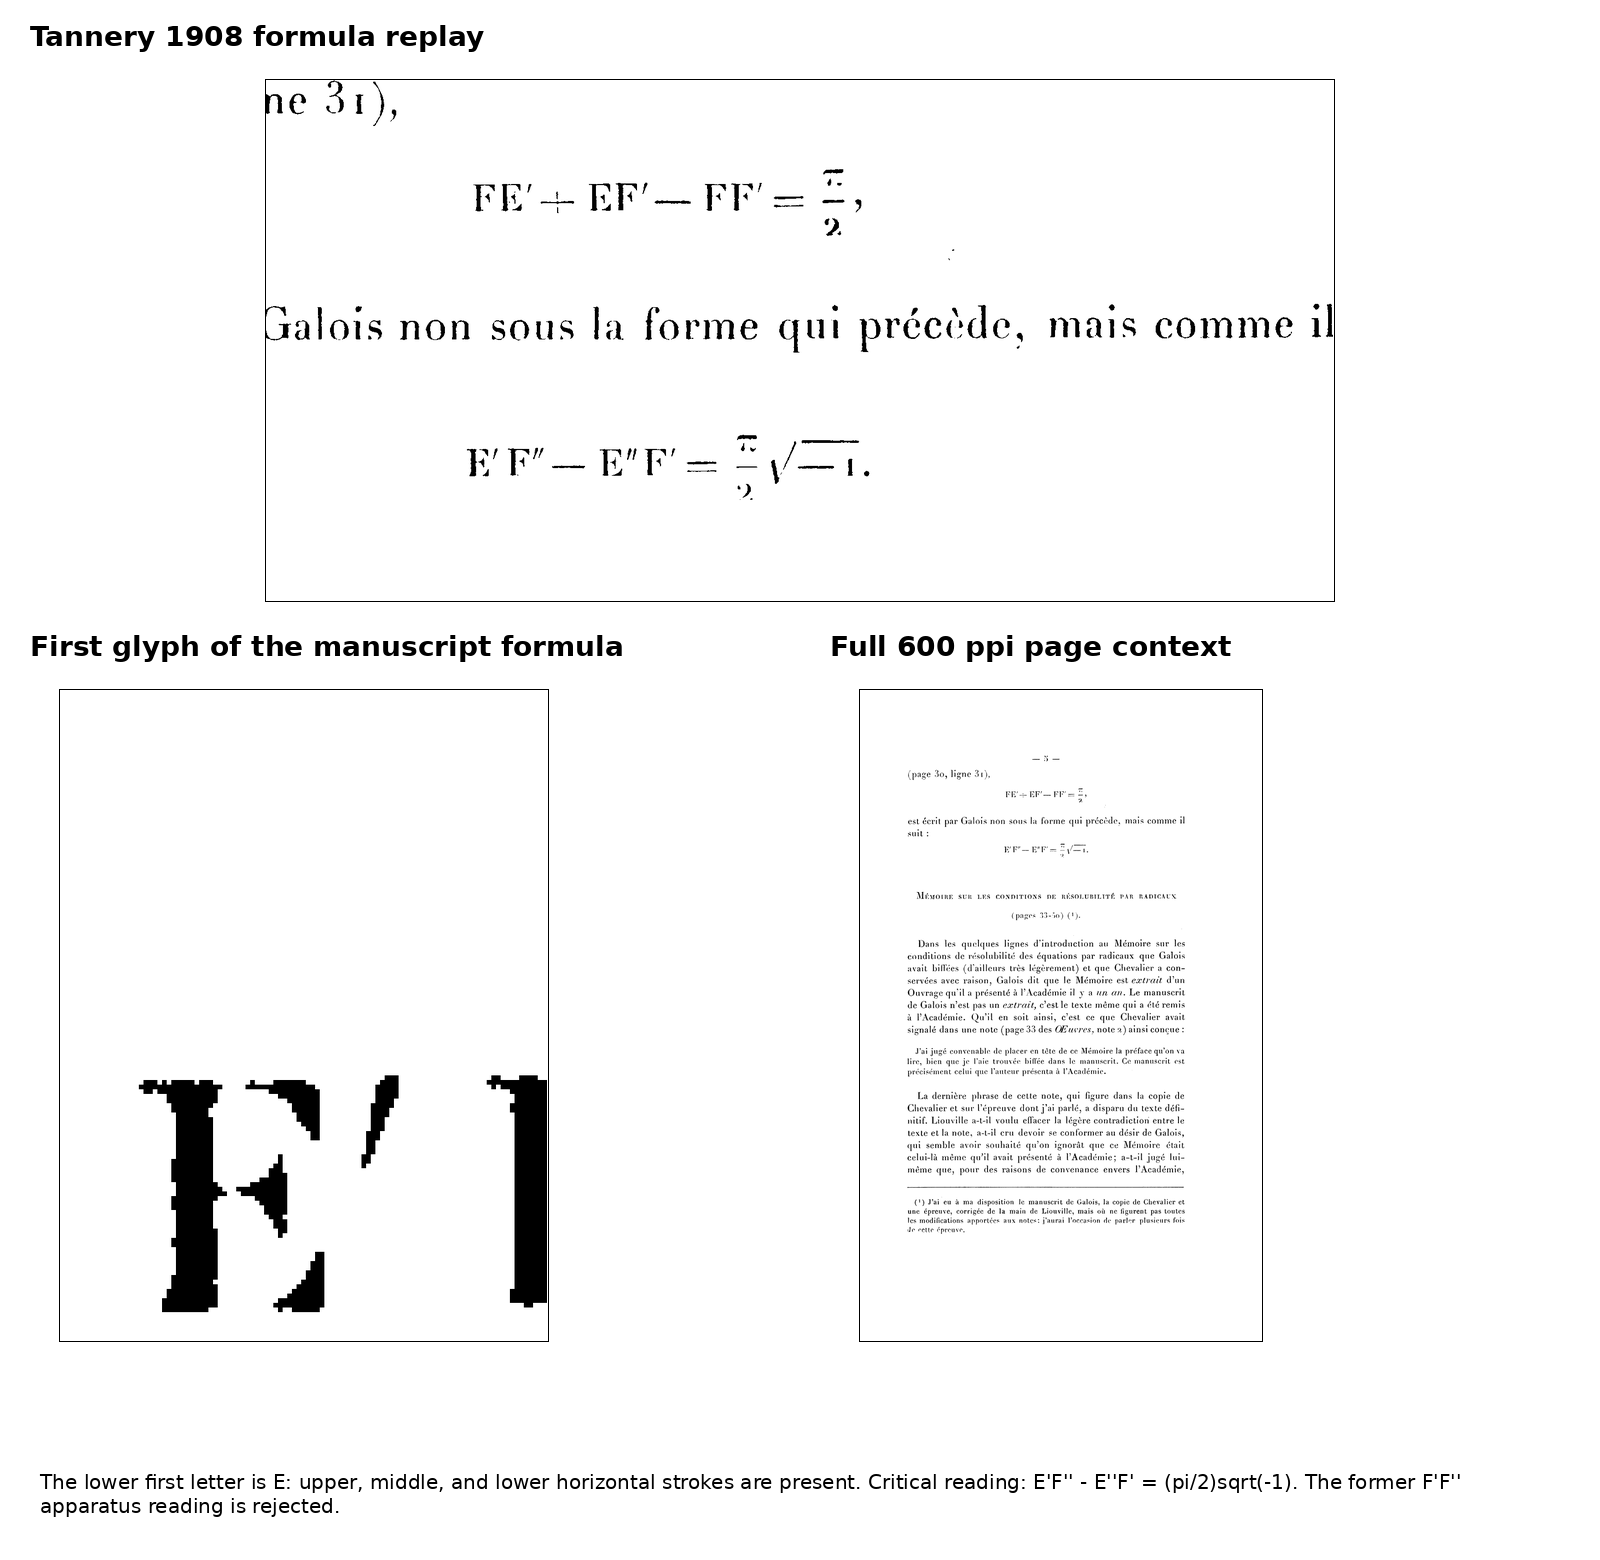
\includegraphics[width=0.95\textwidth,height=\textheight]{../evidence/figures/POST_P13_A008_TANNERY_READING.png}
\caption{Tannery 1908 formula and character replay.}
\end{figure}

\textbf{Theorem (equivalence of the two Legendre forms).} Put

\[
F=K(k),\qquad F_c=K(k'),\qquad E=E(k),\qquad E_c=E(k').
\]

The printed relation is

\[
EF_c+E_cF-FF_c=\frac{\pi}{2}.
\]

Choose the real/imaginary half-period pair and a compatible second-kind
pair by

\[
\omega_1=F,\qquad \omega_2=iF_c,
\qquad
\eta_1=E,\qquad \eta_2=i(F_c-E_c).
\]

Then

\[
\begin{aligned}
\eta_1\omega_2-\eta_2\omega_1
 &=E(iF_c)-i(F_c-E_c)F\\
 &=i(EF_c+E_cF-FF_c)\\
 &=\frac{\pi i}{2}.
\end{aligned}
\]

Identifying Tannery's manuscript symbols by

\[
E'=\eta_1,\qquad F''=\omega_2,\qquad E''=\eta_2,\qquad F'=\omega_1
\]

gives exactly

\[
E'F''-E''F'=\frac{\pi i}{2}.
\]

The chosen second-kind period vector is admissible, not merely an
algebraic relabelling. Start with any second-kind differential having
the same normalized principal part and period vector
\((\widetilde\eta_1,\widetilde\eta_2)\). The Riemann bilinear relation
gives the same determinant \(\pi i/2\). Hence the difference between the
desired vector and the initial vector has zero wedge product with
\(\omega=(\omega_1,\omega_2)\), so it is \(c\omega\) for some constant
\(c\). Adding \(c\) times the holomorphic first-kind differential
realizes exactly the desired period vector.

This identification is compatible with the usual freedom to add a
multiple of a first-kind differential to a second-kind differential:
replacing \(\eta_j\) by \(\eta_j+c\omega_j\) leaves the determinant
invariant, since

\[
(\eta_1+c\omega_1)\omega_2-(\eta_2+c\omega_2)\omega_1
 =\eta_1\omega_2-\eta_2\omega_1.
\]

Thus the manuscript determinant and the 1846/1897 complete-integral
formula express the same Legendre relation under an explicit
half-period/quasi-period normalization. Reversing the orientation of the
second cycle changes the signs of both second-cycle quantities;
Tannery's displayed right-hand side fixes the orientation represented in
his transcription.

\textbf{Historical adjudication.} Tannery 1908 is the earliest securely
dated explicit notice located: he prints both forms and states that
Galois wrote the theorem in the determinant form. DLMF 19.7.1 supplies
the modern complete-integral identity. Beppo Levi's 1927 paper is
explicitly devoted to the half-period/quasi-period determinant
\(\eta_1\omega_2-\eta_2\omega_1=\pi i/2\), confirming that the
determinant normalization is a standard Legendre relation rather than a
different theorem.

\textbf{Propagation.} Neither formula is used in a later deduction in
the 1897 letter. The repair closes the witness-variant task and corrects
the critical apparatus only; it has no downstream change to the
diplomatic edition or to later Galois proofs.

\section{POST-P13-A009 --- W09-PE001 and
W09-PE002}\label{post-p13-a009-w09-pe001-and-w09-pe002}

\textbf{Status:} proved

\textbf{Collation.} At PDF065 the 1897 edition prints ``celle
fonction,'' whereas the 1846 publication prints ``cette fonction.'' At
PDF071 the 1897 edition prints ``proprieté.'' The local 1846 collation
did not establish a comparison reading for that exact token, and no
manuscript-collation source supplies a competing substantive reading.

\textbf{Conclusion.} Both are textual errors: the former is a
demonstrative-agreement error supported by a correct 1846 witness; the
latter is a missing diacritic established from the 1897 spelling and
French orthography. The critical layer restores ``cette fonction'' and
``propriété,'' but records distinct provenance classes. Exact-phrase and
edition searches found no explicit itemized notice; the matrix makes no
novelty claim.

\section{POST-P13-A010 --- W09-SE001 and Lemma
III}\label{post-p13-a010-w09-se001-and-lemma-iii}

\textbf{Status:} repaired

\textbf{Theorem (Bézout repair).} Let K be the coefficient field and V
the separating resolvent. Suppose P(X) and Q(X,V) in K(V){[}X{]} have
exactly one common root a\_i in a splitting field and all relevant roots
are separable. Then a\_i belongs to K(V).

\textbf{Proof.} The monic greatest common divisor D(X)=gcd(P,Q) has
precisely the common roots, hence D(X)=X-a\_i. The Euclidean algorithm
in the PID K(V){[}X{]} gives U(X)P(X)+W(X)Q(X,V)=X-a\_i. Comparing
constant terms, or evaluating the identity in the quotient algebra,
expresses a\_i as an element of K(V). Thus each root singled out by the
resolvent is rational in V.

\textbf{Propagation.} Proposition I's recovery of the roots from V is
now proved. Every later substitution or resolvent construction that
treats the roots as rational functions of V inherits this theorem.
Tannery's 1908 collation reports Galois's own judgment that the
abbreviated proof was insufficient.

\section{POST-P13-A011 --- W09-SE002 and
W09-SE003}\label{post-p13-a011-w09-se002-and-w09-se003}

\textbf{Status:} repaired

\textbf{Theorem (intersection/index).} Let \(L/K\) be the original
splitting field, \(M=K(r)\) an auxiliary extension, \(E=L\cap M\),
\(G=\operatorname{Gal}(L/K)\), and \(H=\operatorname{Gal}(L/E)\). Then
\([G:H]=[E:K]\) and \([E:K]\mid[M:K]\).

\textbf{Proof.} The Galois correspondence gives \([G:H]=[E:K]\). Since
\(E\) is a subfield of \(M\), the tower law gives \([M:K]=[M:E][E:K]\).
If \([M:K]=p\) is prime, the index is \(1\) or \(p\). Without prime
degree the dichotomy is false: \(r=\sqrt2+\sqrt3\) has degree \(4\),
contains \(\mathbf Q(\sqrt2)\), and reduces its \(C_2\) splitting group
with index \(2\).

\textbf{Theorem (Proposition III normality).} If \(M/K\) is also a
splitting field, then \(E/K\) is finite Galois, so \(H\) is normal in
\(G\). Consequently the subgroups arising from conjugate auxiliary roots
coincide after all auxiliary roots are adjoined.

\textbf{Propagation.} These two theorems replace the undefined p and the
omitted proof. They control all dependent group decompositions and the
subsequent radical tower.

\section{POST-P13-A012 --- W09-SE004 Fourier
coefficient}\label{post-p13-a012-w09-se004-fourier-coefficient}

\textbf{Status:} repaired

\textbf{Theorem.} Let θ\_0,\ldots,θ\_\{p-1\} be a nonconstant cyclic
orbit and ζ a primitive p-th root of unity. At least one nontrivial
Fourier coefficient R\_m=Σ\_j ζ\^{}\{mj\}θ\_j, 1≤m≤p-1, is nonzero.

\textbf{Proof.} Fourier inversion gives θ\_j=p\^{}\{-1\}Σ\_m
ζ\^{}\{-mj\}R\_m. If every R\_m for m≠0 vanished, every θ\_j would equal
p\^{}\{-1\}R\_0, contradicting nonconstancy. The printed choice R\_1
need not work: for p=3 and θ\_j=1+ω\^{}j t, one has R\_1=0 but
R\_2=3t≠0.

A cyclic shift multiplies R\_m by a p-th root of unity, so R\_m\^{}p is
invariant. Choosing a nonzero nontrivial coefficient therefore supplies
the intended radical adjunction. The radical-tower conclusion survives
with this selection rule.

\section{POST-P13-A013 --- W09-SE005, W09-SE006, Propositions
VII-VIII}\label{post-p13-a013-w09-se005-w09-se006-propositions-vii-viii}

\textbf{Status:} repaired

\textbf{Counterexample to the unqualified reducibility claim.} The
irreducible polynomial X\^{}3-2 becomes reducible over Q(∛2) but does
not split; the residual quadratic has negative discriminant in the real
embedding. Thus reducibility does not force the group to become trivial
in an arbitrary radical extension.

\textbf{Kummer repair.} Let K contain the relevant p-th roots of unity
and let M/K be an irreducible cyclic Galois Kummer extension of prime
degree p.~For an irreducible polynomial of prime degree n with splitting
field L, put H=Gal(L/L∩M). Then H is normal. Its orbits form a block
system in a prime-degree transitive action, so H is transitive or
trivial. If the polynomial becomes reducible over M, H is not transitive
and is therefore trivial; the polynomial splits completely. This is the
context in which Propositions VI-VII survive.

\textbf{Affine repair.} In Proposition VIII insert ``nonidentity.'' The
identity k↦k fixes every letter; a nonidentity affine map k↦ak+b fixes
at most one. Hence adjoining two roots kills every nonidentity group
element, and the final affine necessity/sufficiency argument survives.

\section{POST-P13-A014 --- W09 provenance
corpus}\label{post-p13-a014-w09-provenance-corpus}

\textbf{Status:} proved

This certificate belongs to the critical layer. The P13R diplomatic
transcription and its 78-page PDF are immutable. No wording below
authorizes a silent change to that layer. Coordinates are physical
PDF/JP2 coordinates from the frozen map.

The six W09 witness variants are all explicitly grounded in Tannery's
1908 collation: omitted definitions, Lemma III's insufficiency, deletion
of the prime-degree phrase, the revised Proposition III, a marginal
construction sentence, and the expanded Cauchy citation. The 1846
witness supplies the correct form for W09-PE001; W09-PE002 is diagnosed
from the 1897 spelling itself, without a securely established 1846
comparison token. The 1962 critical edition is bibliographically
verified; a 1977 review verifies that the 1976 facsimile printing added
supplementary pages containing an errata list and two concordances, but
the item-level entries were inaccessible. Neumann's 2011 book has a
corrected second printing dated September 2013. Dicker's paper submitted
July 22, 2026 specifically reconstructs Proposition II, not Lemma III or
Proposition III.

The matrix records these as established prior art where direct evidence
exists. W09-SE004--006 are recorded as ``no prior notice found in the
searched corpus,'' not as new results.

\section{W10-DA001 --- prime-power theorem and unique
blocks}\label{w10-da001-prime-power-theorem-and-unique-blocks}

\textbf{Status:} repaired

\textbf{Theorem.} A finite solvable primitive permutation group G has
degree p\^{}d and embeds in AGL(d,p).

\textbf{Proof.} Choose a minimal nontrivial normal subgroup N of G.
Solvability makes N elementary abelian of order p\^{}d.~The N-orbits
form a G-invariant block system; primitivity makes N transitive. Since N
is abelian, a point stabilizer N\_α is normal in G: all point
stabilizers in N are equal by abelianness and their intersection is the
kernel of the faithful action, hence trivial. Thus N is regular.
Identifying the points with N gives an affine space over F\_p.~A point
stabilizer H acts faithfully by conjugation on N and is irreducible,
because an H-invariant proper nonzero subgroup of N would yield a
nontrivial block system. Hence G=N⋊H≤AGL(d,p).

\textbf{Disposition.} The printed unique-block construction is
incomplete but its prime-power conclusion survives under the inherited
finite solvable primitive hypotheses.

\section{W10-DA002 --- affine
linearity}\label{w10-da002-affine-linearity}

\textbf{Status:} repaired

\textbf{Qualified theorem.} Under the inherited hypotheses that the
permutation group is finite, solvable, and primitive of degree p\^{}d,
W10-DA001 identifies the letters with the regular elementary-abelian
socle V and identifies the point stabilizer with an irreducible subgroup
of GL(V). Every group element is therefore affine: x↦Ax+b.

\textbf{Failure of the unqualified reading.} Primitivity alone does not
imply affine linearity. For example, S\_\{p\^{}2\} in its natural action
is primitive, but for p\^{}2≥5 it has nonabelian simple socle
A\_\{p\^{}2\} and no regular elementary-abelian normal subgroup. It
cannot be an affine group of degree p\^{}2.

\textbf{Conclusion.} Formula (A), after W10-PE005 is repaired, is valid
only inside the inherited solvable-primitive argument.

\section{W10-DA003 --- PDF089 conjuguées and pairwise
equality}\label{w10-da003-pdf089-conjuguuxe9es-and-pairwise-equality}

\textbf{Status:} rejected

\textbf{Historical finding.} Cauchy's technical phrase ``système de
substitutions conjuguées'' designated what modern historians translate
as a ``system of conjoined substitutions,'' namely a substitution system
closed under composition; Hollings explicitly warns that the translation
``conjugate substitutions'' is best avoided because of its modern
group-theoretic meaning. In the PDF089 sentence, the immediately
preceding clause already says that the substitutions are transformed
into one another by the translations ((k,k+m)). Thus the historically
supportable force is membership in, or transport within, the relevant
closed substitution system/orbit---not pairwise commutativity. The
lexical evidence does not establish a stronger relation.

\textbf{Exact counterexample in the printed projective family.} On
P\^{}1(F\_7), set T\_m(k)=m+1/(k-m), with the usual values at infinity.
Translation τ\_1 conjugates T\_0 to T\_1. Nevertheless direct evaluation
shows T\_0T\_1≠T\_1T\_0. Thus even two members related by the evident
translation conjugacy fail to commute.

\textbf{Consequence.} Neither the historically attested
``conjoined-system'' sense nor modern element conjugacy implies pairwise
commutativity. The premise used at PDF089 is therefore unsupported;
under modern conjugacy it is explicitly false. The terminal p=3
conclusion depending on it is blocked. No diplomatic wording is changed.

\section{\texorpdfstring{W10-DA004 --- propagation through the
\(p\)-power and \(p^2\)
arguments}{W10-DA004 --- propagation through the p-power and p\^{}2 arguments}}\label{w10-da004-propagation-through-the-p-power-and-p2-arguments}

\textbf{Status:} repaired

W10-PE001--PE004 restore the coordinate tuples and maps on PDF082--083.
W10-PE005 restores the two-dimensional affine formula; with
W10-DA001--002 it expresses the solvable primitive group as an affine
group. W10-SE001 adds the nonidentity qualification to the fixed-space
dimension count; its divisibility conclusion survives. W10-SE002 changes
only the count of fixed-point-free nonidentity scalars from \(p^2-1\) to
\(p^2-2\); the scalar subgroup order \(p^2-1\) and total affine group
order \(p^2(p^2-1)(p^2-p)\) survive. W10-PE006 restores the projective
fixed-point equation and makes the printed discriminant correct, so the
support-size trichotomy survives.

The final PDF089 pairwise-commutativity premise does not survive, by
W10-DA003. Accordingly, the p=3 terminal inference is not carried into
the corrected theorem set.

\section{W11-DA001 --- table-of-contents 1 to
v}\label{w11-da001-table-of-contents-1-to-v}

\textbf{Status:} proved

The frozen page map and the primary 1897 images place Picard's
Introduction on roman folios v-x. The 1897 table of contents
nevertheless prints Arabic 1. An independent Harvard-copy Wikisource
transcription prints v; its permanent page record states that the page
was last modified on July 22, 2018. This is the earliest securely dated
correction located in the accessible corpus.

The official ETH-Bibliothek copy, shelfmark Rar 4575 and DOI
10.3931/e-rara-19915, was subsequently retrieved at page level. Its
table of contents independently prints the same Arabic \texttt{1},
showing that the error belongs to the 1897 printed edition rather than
to the canonical scan alone. The 1976 Bourgne--Azra printing is known to
add an errata list, but that item-level list was not accessible, so no
earlier notice is attributed to it.

\section{W11-DA002 --- printer job
number}\label{w11-da002-printer-job-number}

\textbf{Status:} proved

\textbf{Independent witness.} The official ETH-Bibliothek digitization
of the independent 1897 copy, shelfmark Rar 4575 and DOI
10.3931/e-rara-19915, was retrieved from the library's public download
endpoint. Its PDF page 79 contains the colophon. The small printer
number to the left of the second line is visibly

{[} \boxed{24572}. {]}

It has five digits, not four. The official ETH OCR independently
transcribes \texttt{24572} on the same colophon page.

\begin{figure}
\centering
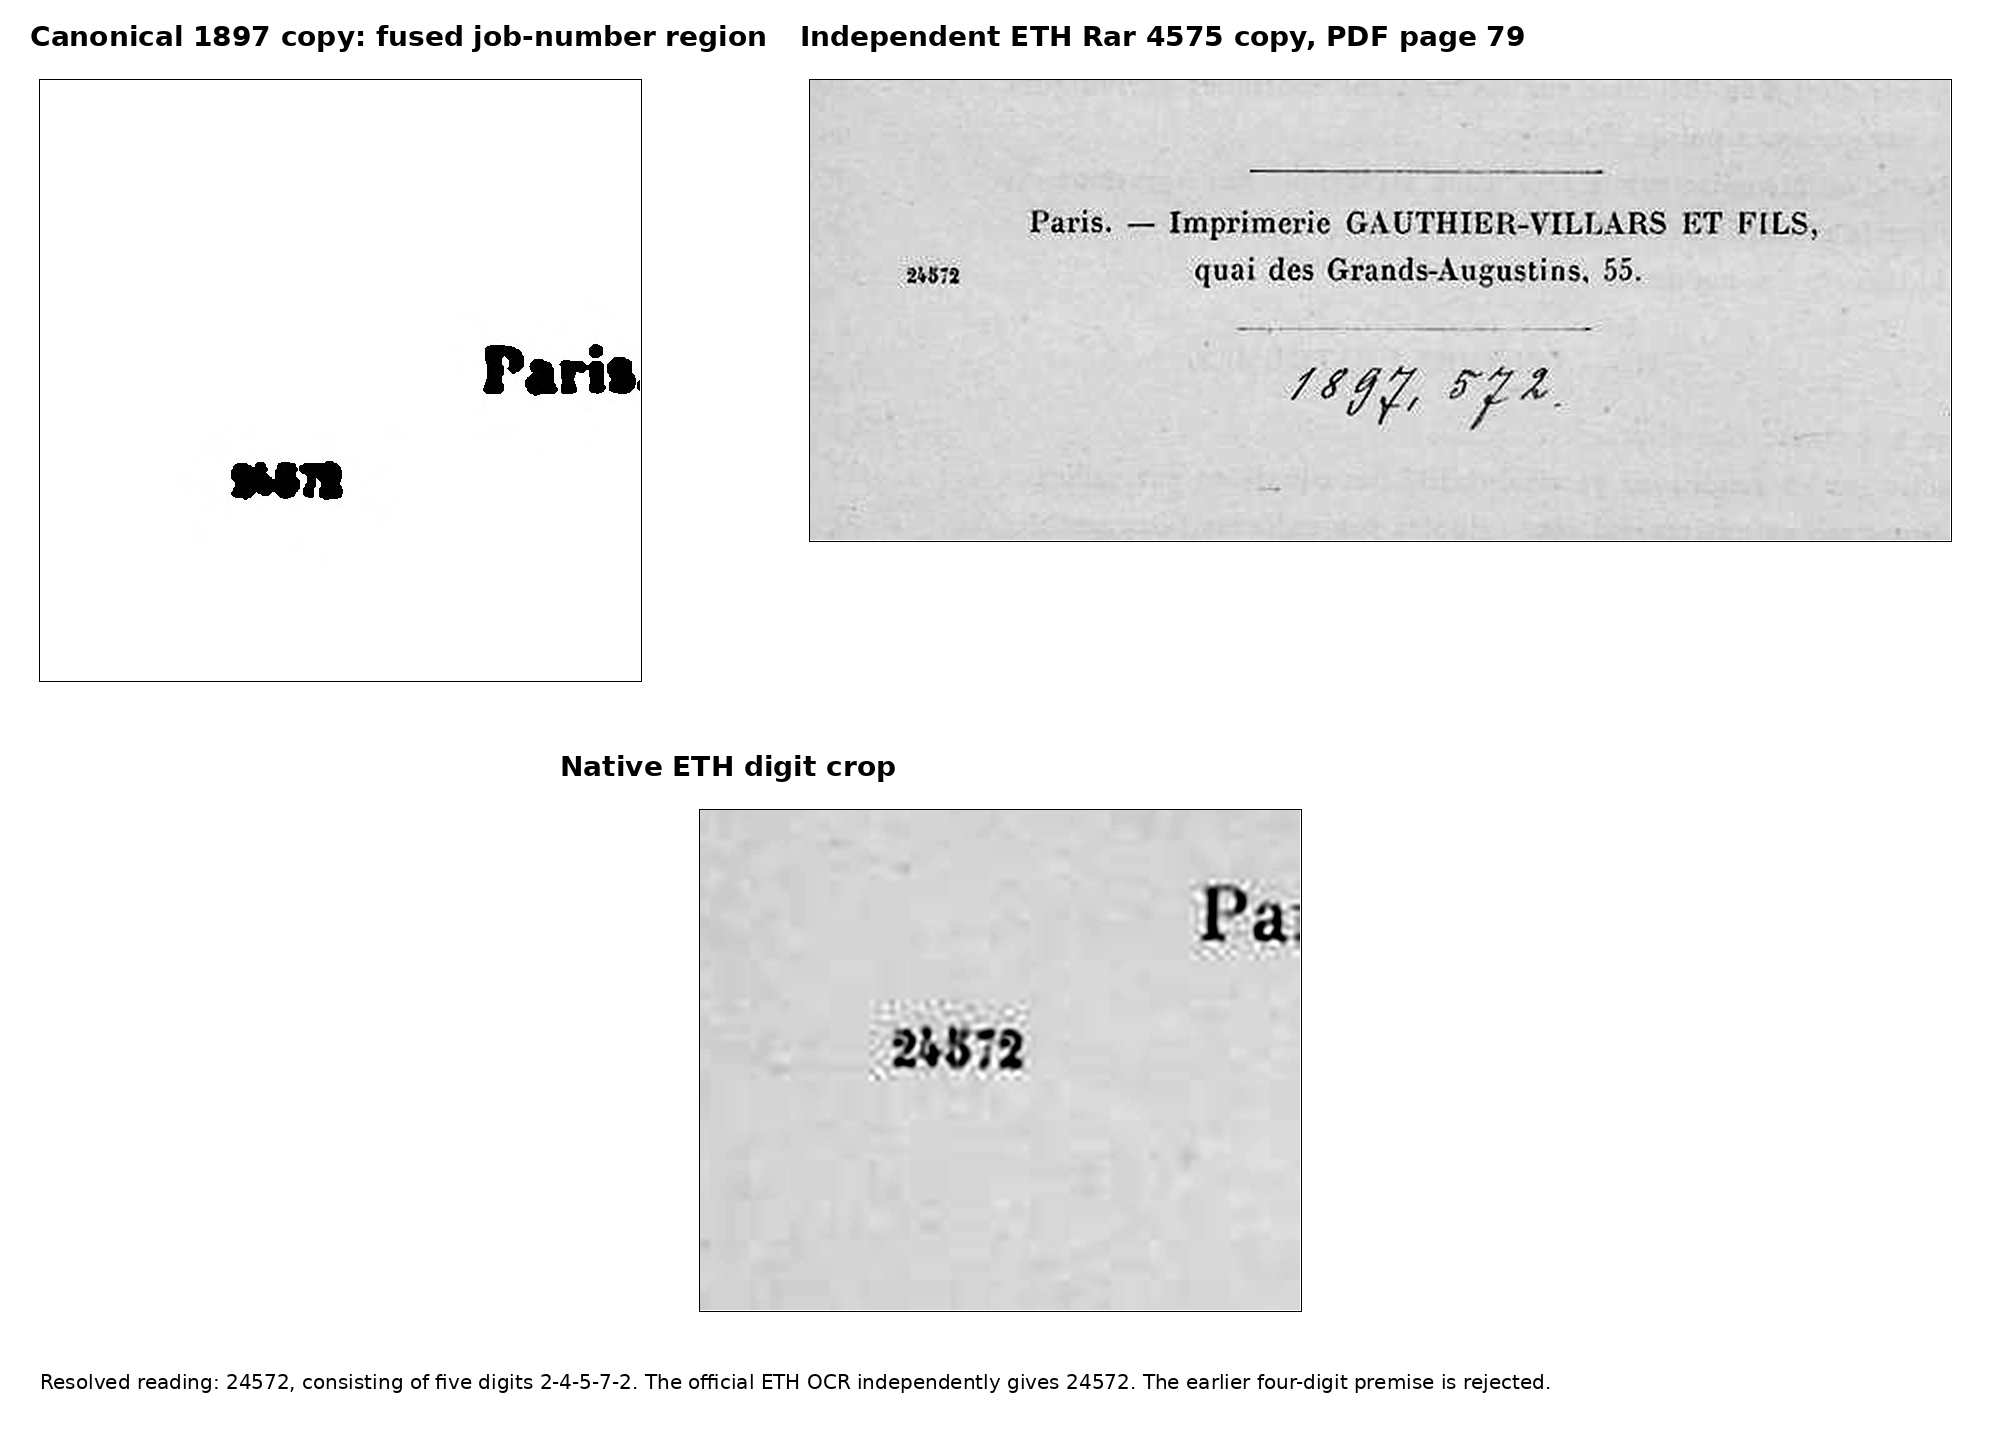
\includegraphics[width=0.95\textwidth,height=\textheight]{../evidence/figures/W11_DA002_JOB_NUMBER_COMPARISON.png}
\caption{Canonical and ETH colophon comparison.}
\end{figure}

\textbf{Character-by-character certificate.} In the independent image,
the first and fifth glyphs have the curved upper stroke, diagonal
descent, and basal stroke of \texttt{2}; the second has the vertical and
cross-stroke structure of \texttt{4}; the third has the top bar and
lower bowl of \texttt{5}; and the fourth has a top bar with descending
diagonal, hence \texttt{7}. The sequence is therefore
\texttt{2-4-5-7-2}. The canonical JP2 remains locally fused, but its
five dark glyph components are consistent with the independent reading.
The independent image, rather than the OCR alone, is decisive.

\textbf{Disposition.} \texttt{W11-U001} is closed in the critical layer
with reading \texttt{24572}. The historical 1897 diplomatic page is not
re-typeset or silently altered; the critical appendix and
machine-readable resolution ledger carry the reading and evidence. No
Gauthier-Villars printer register was needed after recovery of the
independent comparison copy.

\section{W11-DA003 --- terminal topology and P10/P11
boundary}\label{w11-da003-terminal-topology-and-p10p11-boundary}

\textbf{Status:} proved

Replay of the primary PDF, JP2 leaves, disposition map, and integrated
candidate gives the following exact topology: PDF091/L0090 is the
predecessor blank owned by W10; PDF092/L0091 is the historical table of
contents; PDF093/L0092 is the colophon; PDF094/L0093, PDF095/L0094, and
PDF096/L0095 are three distinct trailing blanks. The P10/P11 boundary
introduces no text join. The corrected critical page reference v does
not alter the historical table in the diplomatic layer.

All six physical leaves remain dispositioned exactly once. The one-click
reader preserves the frozen 78-page diplomatic PDF as its prefix; the
critical appendix follows it and does not collapse any blank topology.

\section{Resolved after the R2 deep
replay}\label{resolved-after-the-r2-deep-replay}

Two records formerly marked \texttt{unresolved\_after\_bounded\_search}
are now closed:

\begin{longtable}[]{@{}
  >{\raggedright\arraybackslash}p{(\columnwidth - 4\tabcolsep) * \real{0.3333}}
  >{\raggedright\arraybackslash}p{(\columnwidth - 4\tabcolsep) * \real{0.3333}}
  >{\raggedright\arraybackslash}p{(\columnwidth - 4\tabcolsep) * \real{0.3333}}@{}}
\toprule\noalign{}
\begin{minipage}[b]{\linewidth}\raggedright
record\_id
\end{minipage} & \begin{minipage}[b]{\linewidth}\raggedright
R2 status
\end{minipage} & \begin{minipage}[b]{\linewidth}\raggedright
resolution
\end{minipage} \\
\midrule\noalign{}
\endhead
\bottomrule\noalign{}
\endlastfoot
W08-WV001 / POST-P13-A008 & repaired & The first manuscript glyph is
\texttt{E}, and the determinant form is proved equivalent to the printed
Legendre relation under an explicit period normalization. \\
W11-U001 / W11-DA002 & proved & The independent ETH 1897 copy and OCR
give the five-digit printer job number \texttt{24572}. \\
\end{longtable}

\section{Open readings after the R2 deep
replay}\label{open-readings-after-the-r2-deep-replay}

Three records remain open. They are inherited W01 image/provenance
questions outside the mathematical 21-task scope; neither post-P13 task
remains unresolved.

\begin{longtable}[]{@{}
  >{\raggedright\arraybackslash}p{(\columnwidth - 4\tabcolsep) * \real{0.3333}}
  >{\raggedright\arraybackslash}p{(\columnwidth - 4\tabcolsep) * \real{0.3333}}
  >{\raggedright\arraybackslash}p{(\columnwidth - 4\tabcolsep) * \real{0.3333}}@{}}
\toprule\noalign{}
\begin{minipage}[b]{\linewidth}\raggedright
record\_id
\end{minipage} & \begin{minipage}[b]{\linewidth}\raggedright
status
\end{minipage} & \begin{minipage}[b]{\linewidth}\raggedright
missing evidence
\end{minipage} \\
\midrule\noalign{}
\endhead
\bottomrule\noalign{}
\endlastfoot
W01-U001 & carried forward unresolved outside 21-task scope & A
character-resolved independent image or documented portrait-plate source
sufficient to read the faint lower-left signature on PDF019. \\
W01-U002 & carried forward unresolved outside 21-task scope &
Independent provenance evidence sufficient to adjudicate the relation
between the degraded PDF021 portrait and PDF019 without silently
deduplicating witnesses. \\
W01-U003 & carried forward unresolved outside 21-task scope & A
higher-fidelity device image or printer-source record sufficient to
expand the publisher-device ribbon legend character by character. \\
\end{longtable}

\section{Historical-priority
conclusions}\label{historical-priority-conclusions}

Direct evidence establishes Liouville's 1846 footnote as notice of the
p=7 and p=11 modular exceptions; Tannery's 1908 collation as explicit
notice of multiple W08-W10 editorial and proof defects; the 1976
Bourgne-Azra printing as containing an added errata list whose
item-level contents were unavailable; and the Harvard-copy Wikisource
page as a dated silent correction of the contents reference to roman v
on July 22, 2018. All other negative findings are stated only as ``no
prior notice found in the searched corpus.''

\section{Bibliographic sources}\label{bibliographic-sources}

\begin{itemize}
\tightlist
\item
  \textbf{SRC-LOCAL-1897.} Évariste Galois; Société mathématique de
  France; introduction by Émile Picard, \emph{Œuvres mathématiques
  d'Évariste Galois} (1897), Paris: Gauthier-Villars et Fils, physical
  PDF 1-96; printed x, 1-61 plus back matter.
\item
  \textbf{SRC-LOCAL-1846.} Évariste Galois; edited by Joseph Liouville,
  \emph{Œuvres mathématiques} (1846), Journal de Mathématiques Pures et
  Appliquées, série 1, vol.~11, 381-444; local PDF 1-65.
  \url{https://www.numdam.org/item/JMPA_1846_1_11__381_0/}
\item
  \textbf{SRC-LOCAL-1908.} Jules Tannery, editor, \emph{Manuscrits
  d'Évariste Galois} (1908), Paris: Gauthier-Villars, local PDF 1-77;
  Commons scan 87 leaves.
  \url{https://commons.wikimedia.org/wiki/File:Galois_-_Manuscrits,_édition_Tannery,_1908.djvu}
\item
  \textbf{SRC-NUMDAM-1846.} Numdam, \emph{Numdam record for the 1846
  publication} (1846/online), Numdam item: JMPA 1846, series 1, volume
  11, page 381, 381-444; record marks corrected-by Errata.
  \url{https://www.numdam.org/item/JMPA_1846_1_11__381_0/}
\item
  \textbf{SRC-ETH-1897.} ETH-Bibliothek Zürich, \emph{ETH-Bibliothek
  independent copy of Oeuvres mathématiques} (1897; online 2013-10-08),
  Rar 4575; DOI 10.3931/e-rara-19915, X, 61 pages, one leaf.
  \url{https://www.e-rara.ch/zut/content/titleinfo/6262819}
\item
  \textbf{SRC-WIKI-1897.} French Wikisource contributors, \emph{Harvard
  College Library 1897 copy transcription} (1897 scan; current online
  transcription), Gauthier-Villars 1897, complete index.
  \url{https://fr.wikisource.org/wiki/Livre:Galois_-_Œuvres_mathématiques,_Gauthier-Villars,_1897.djvu}
\item
  \textbf{SRC-WIKI-TOC.} French Wikisource contributors, \emph{1897
  table-of-contents transcription, page 91} (last modified 2018-07-22),
  oldid 7722271, page 91.
  \url{https://fr.wikisource.org/w/index.php?title=Page:Galois_-_Œuvres_mathématiques,_Gauthier-Villars,_1897.djvu/91&oldid=7722271}
\item
  \textbf{SRC-DLMF-LEGENDRE.} NIST Digital Library of Mathematical
  Functions, \emph{DLMF §19.7(i), Legendre's Relation} (current
  reference), Equation 19.7.1, §19.7(i).
  \url{https://dlmf.nist.gov/19.7.E1}
\item
  \textbf{SRC-BDIM-LEGENDRE-1927.} Beppo Levi, \emph{Sulla relazione
  \(\eta_1\omega_2-\eta_2\omega_1=\pi i/2\) nella teoria delle funzioni
  ellittiche} (1927), \emph{Bollettino dell'Unione Matematica Italiana},
  series 1, vol.~6, no. 3, pp.~137-141.
  \url{https://www.bdim.eu/item?id=BUMI_1927_1_6_3_137_0}
\item
  \textbf{SRC-BOURGNE-AZRA-1962.} Robert Bourgne and Jean-Pierre Azra,
  editors, \emph{Écrits et mémoires mathématiques d'Évariste Galois}
  (1962), Gauthier-Villars; xxii+541 pp., critical edition.
  \url{https://doi.org/10.1017/S0008439500026989}
\item
  \textbf{SRC-BOURGNE-AZRA-1976.} Robert Bourgne and Jean-Pierre Azra,
  editors, \emph{Écrits et mémoires mathématiques d'Évariste Galois, 2e
  éd.} (1976), new facsimile printing with supplementary errata and two
  concordances, xxxi+541 pp..
  \url{https://www.persee.fr/doc/rhs_0151-4105_1977_num_30_2_1486}
\item
  \textbf{SRC-NEUMANN-2013.} Peter M. Neumann, \emph{The mathematical
  writings of Évariste Galois} (2011; corrected second printing
  September 2013), EMS Heritage of European Mathematics 104, 1-410.
  \url{https://ems.press/books/hem/102/contents}
\item
  \textbf{SRC-DICKER-2026.} Math Dicker, \emph{The Significance of
  Proposition II in Galois' Mémoire, The Origin of Galois Automorphisms}
  (2026-07-22), arXiv:2607.20147, abstract and paper.
  \url{https://arxiv.org/abs/2607.20147}
\item
  \textbf{SRC-CAUCHY-TERMS.} Christopher D. Hollings, \emph{`Nobody
  could possibly misunderstand what a group is': a study in early
  twentieth-century group axiomatics} (2017), Archive for History of
  Exact Sciences 71, 409--481, especially §2.1 on early substitution
  terminology. \url{https://doi.org/10.1007/s00407-017-0193-8}
\item
  \textbf{SRC-AFFINE-PRIMITIVE.} Attila Maróti and Saveliy V. Skresanov,
  \emph{Bounds for the Diameters of Orbital Graphs of Affine Groups}
  (2023), Vietnam Journal of Mathematics 51, 617--631; introductory
  definition of affine primitive groups.
  \url{https://doi.org/10.1007/s10013-023-00607-5}
\item
  \textbf{SRC-LI-2003.} Cai Heng Li, \emph{The Finite Primitive
  Permutation Groups Containing an Abelian Regular Subgroup} (2003),
  Proc. London Math. Soc. 87, 725-747.
  \url{https://doi.org/10.1112/S0024611503014266}
\end{itemize}

\section{Machine-readable companions}\label{machine-readable-companions}

The authoritative structured companions are
\texttt{MASTER\_21\_TASK\_LEDGER.csv},
\texttt{CRITICAL\_ERRATA\_CATALOGUE.csv},
\texttt{BIBLIOGRAPHIC\_PRIOR\_NOTICE\_MATRIX.csv},
\texttt{SEARCH\_QUERY\_LEDGER.csv},
\texttt{DEPENDENCY\_PROPAGATION\_EDGES.csv}, the frozen and R2
resolution/open ledgers, and \texttt{qa/MATHEMATICAL\_CHECKS.json}.

\end{document}
